\section{Introduction}\label{sec:intro}

%\subsection{Online Video Games}\label{sec:onlinevideogames}

%\emph{League of Legends} (LoL) is an online multiplayer game created by \emph{Riot Games} (Riot). In 2015 LoL was the most played game in the world, with more then 27 million daily players~\cite{LoL27mill}~\cite{LoLmostplayed} .Each player is considered a \emph{summoner}, who has access to \emph{masteries} and \emph{runes} which are selectable additions, used to improve the user controlled \emph{champions}. In a classic 5 versus 5 match, 10 players are divided into the two competing teams; blue and purple. Each player will pick a champion, from a pool of 124 unique champions. Each champion has 5 unique abilities; four actives and one passive. Out of the four actives, one is an ultimate that is extra powerful. Passive abilities cannot be activated by the player. which means it is always active. An \emph{ability} is a magic spell, which does wildly different things, e.g. frost shots that deal damage and slow units, or heals that replenishes health points on target units.

\emph{League of Legends} (LoL) is a PC game created by \emph{Riot Games} (Riot). In the beginning of 2014 LoL had 27 million daily players~\cite{LoL27mill}. One year later it was the most played multiplayer game in the world~\cite{LoLmostplayed}. 
%The game clearly gathers a lot of attention, but not much research in the area of computer science has been published about the game. 
In the following we will explain the mechanics of the game, and identify a problem which will be the focus of this project. 

In a classic 5 versus 5 match, 10 players are divided into two competing teams consisting of 5 players each, with the colours blue and purple. Each player is considered a \emph{summoner}, who has access to \emph{masteries} and \emph{runes}, which improve the \emph{champions}. In addition, a summoner has access to \emph{summoner spells}, which are global for all champions available to that summoner. Before a match can begin, each player picks a champion from a pool of 124, to use as their playable character. Each champion has 5 unique abilities: The ultimate which is extra powerful, three activatable abilities and lastly one passive ability, examples of abilities can be seen in \Cref{fig:ashe}.

\begin{figure}[!htb]
  \centering
  \begin{subfigure}[b]{0.49\textwidth}
    \includegraphics[width=\textwidth]{img/frostshot.png}
    \caption{Example of a passive ability}\label{fig:frostshot}
  \end{subfigure}
  \begin{subfigure}[b]{0.49\textwidth}
    \includegraphics[width=\textwidth]{img/volley.png}
    \caption{Example of an active ability}\label{fig:volley}
  \end{subfigure}
  \begin{subfigure}[b]{0.49\textwidth}
    \includegraphics[width=\textwidth]{img/enchanted.png}
    \caption{Example of an ultimate ability}\label{fig:enchanted}
  \end{subfigure}
  \caption{Subset of Ashe's skillset~\cite{ashe}}\label{fig:ashe}
\end{figure}

In \Cref{fig:lolmap} the map of the game can be seen. The map consists of three lanes identified as \emph{top}, \emph{middle}, and \emph{bottom} which connects the two bases. The blue and purple colours represent the blue and purple teams' respective structures. Circles are \emph{turrets}, pentagons are \emph{inhibitors}, and squares are each team's \emph{nexus}. The green circle indicates \emph{the dragon} and the pink is \emph{the baron}.

\begin{description}
\item[Nexus:] This building spawns \emph{creeps}, which are small monsters with low damage and health, that walks along each of the lanes toward the opposing teams base. Killing the creeps award \emph{gold} and \emph{experience}. When the nexus is destroyed the game ends, making the destroying team the winners.
\item[Inhibitor:] When this building is destroyed, the destroying teams' minions become stronger on the lane where the inhibitor was.
\item[Turret:] This is a defensive structure, which fires at nearby enemies.
\item[Jungle:] The area between the lanes which hosts neutral monsters, that awards gold and experience when killed.
\end{description}

\begin{figure}[!htb]
  \centering
    \includegraphics[width=0.6\textwidth]{img/lolmap.jpg}
  \caption{League of Legends map~\cite{lolmap}}\label{fig:lolmap}
\end{figure}

Due to the fact that creeps are spawned at both bases at the same time, they will meet at the middle of the lanes, where the majority of the fighting will take place. The dragon is a strong monster, which grants a team a permanent attribute bonus when killed. The baron resembles the dragon, but the attribute bonus is a lot stronger and temporary.

Experience and gold are the currencies of the game, which are earned by killing creeps, monsters, or opposing champions. Both are earned individually by each player. Experience is used to improve the abilities of the champion, while gold is spent purchasing items, that will make the champion more powerful. The game is thus an ever-evolving battle of killing the most units, pushing towards the enemies base, and winning team fights. Usually one team will accumulate an advantage by being ahead in gold, experience, or both. This makes their champions stronger, making it easier to win fights. When one team is ahead, the other team must play more carefully, adjust abilities, items, and utilising their champions correctly to turn the deficit.

\begin{figure}[!htb]
  \centering
    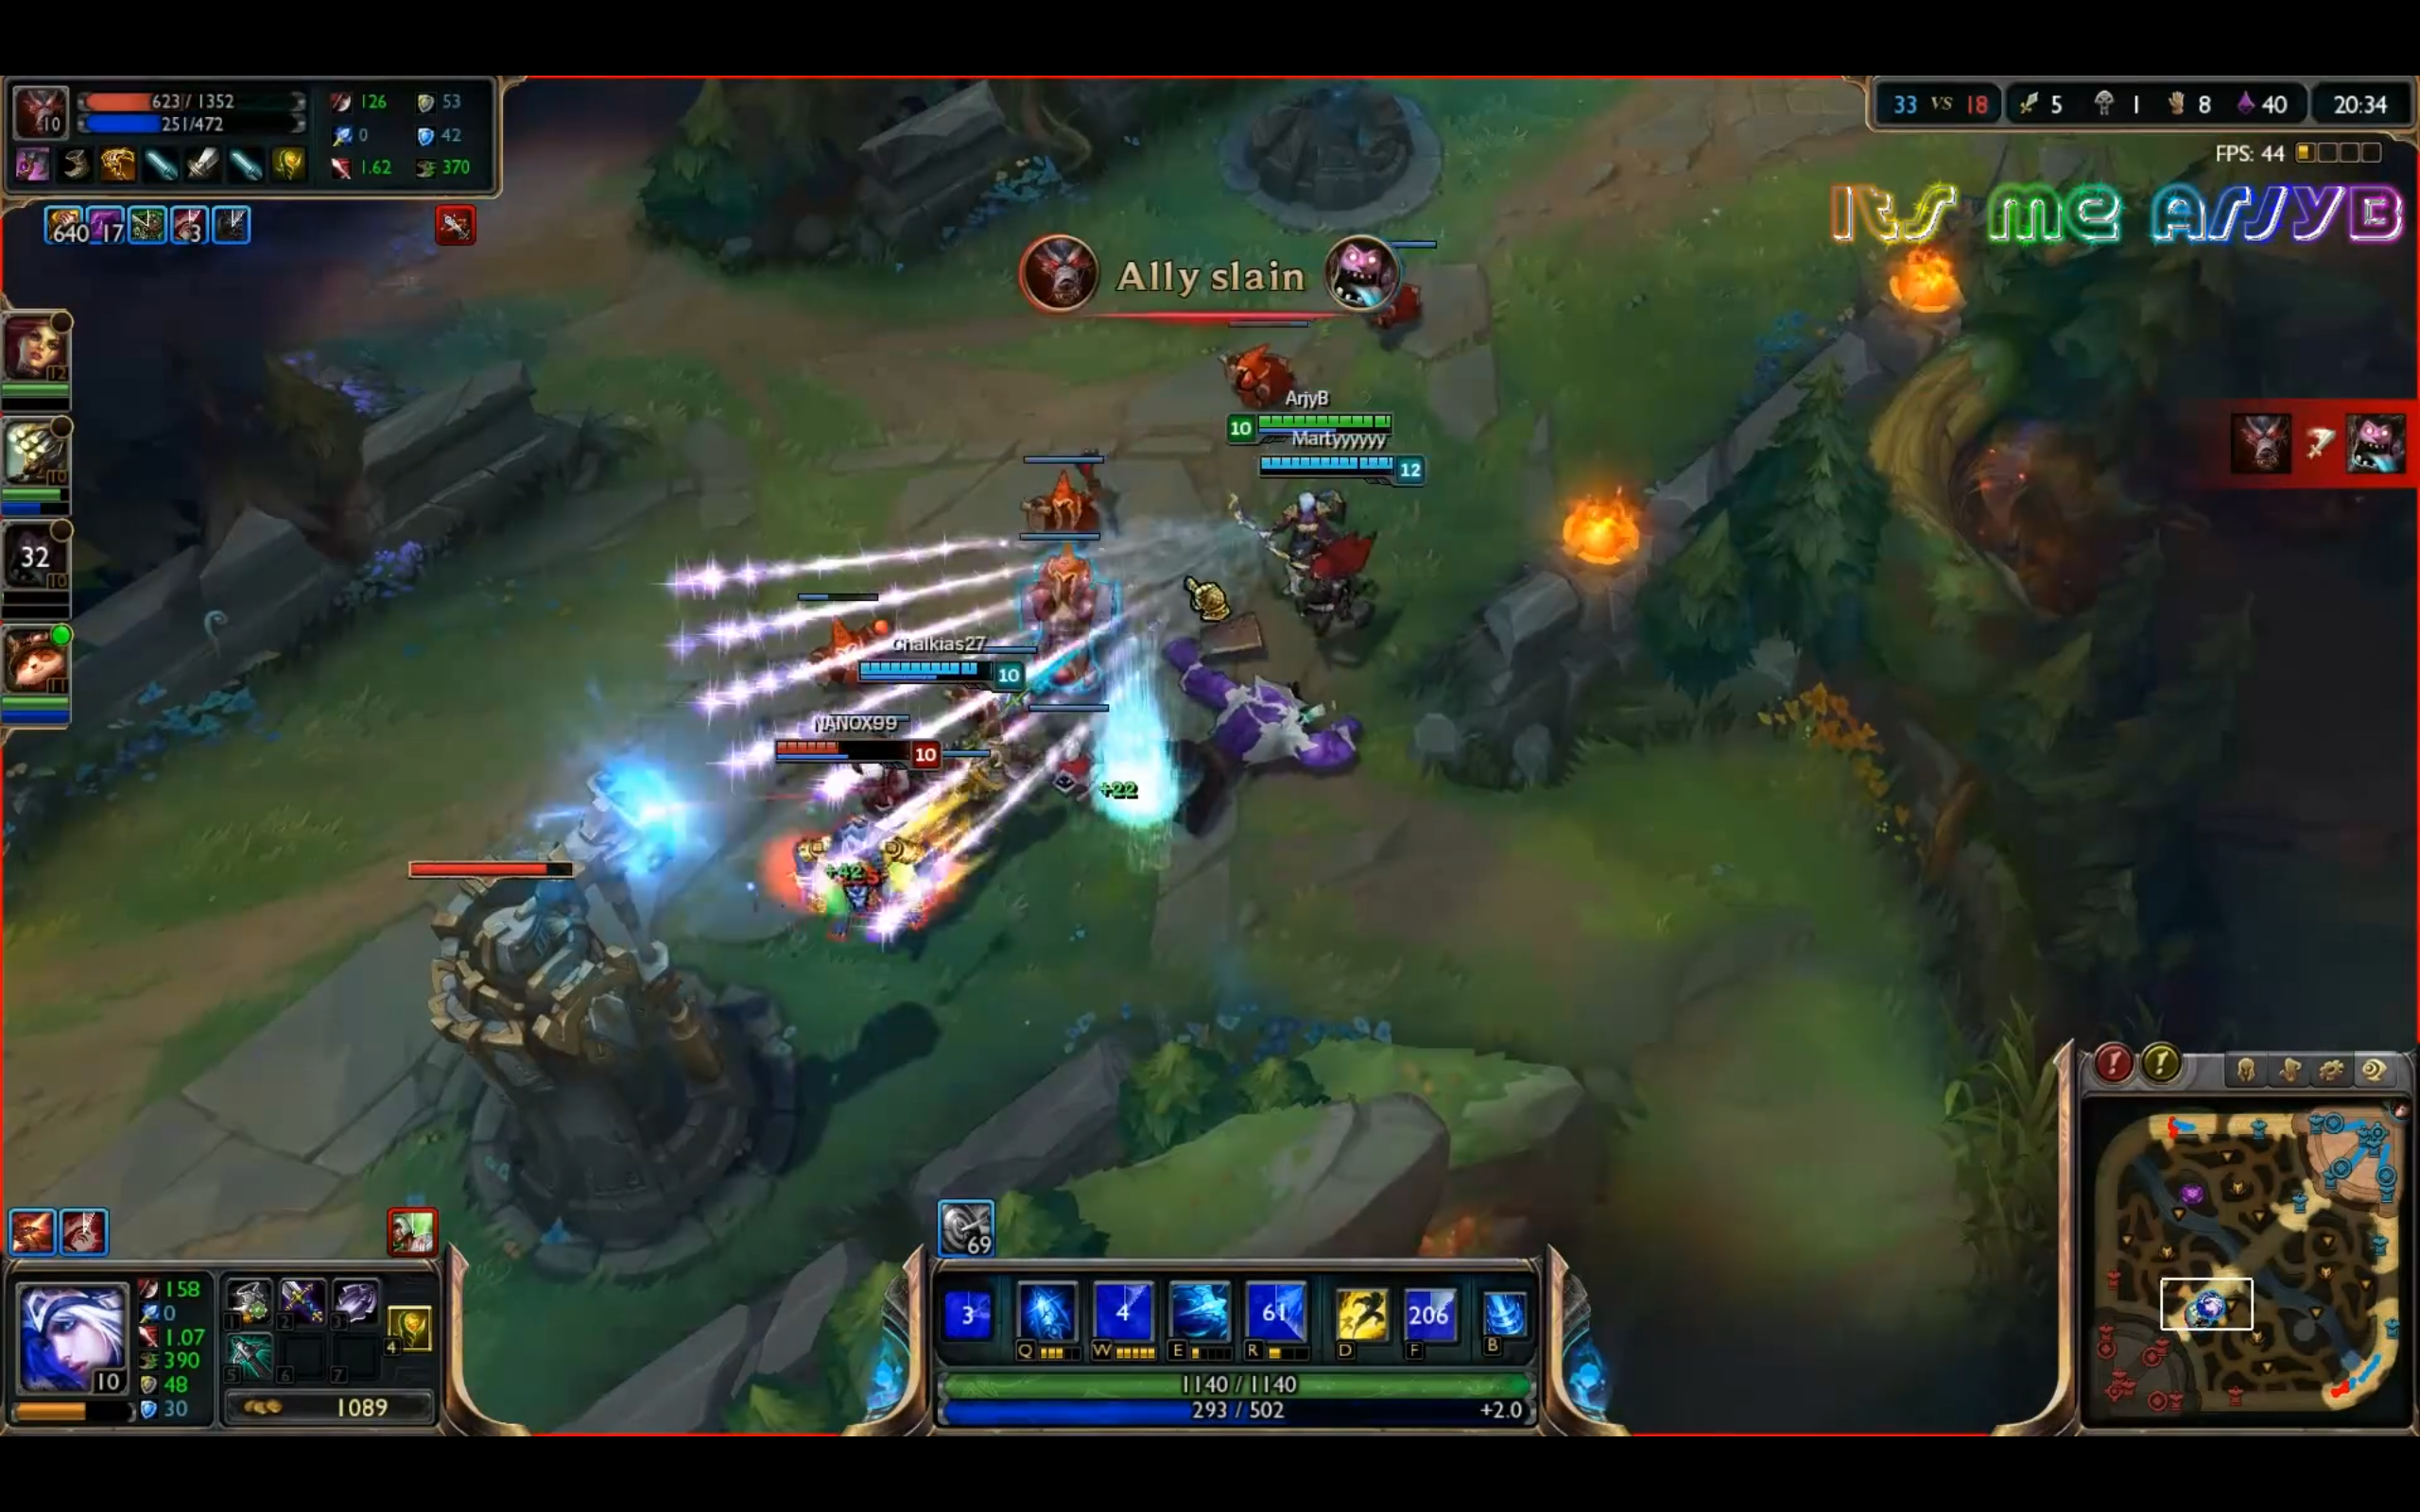
\includegraphics[width=1\textwidth]{img/lolgame.png}
  \caption{Screenshot of an ongoing match: Lower left corner shows the player's champion equipment and stats. Upper left corner shows team information as well as a summary of a selected champion. Upper right corner shows the current score of the game. The lower right corner shows the map. Lastly the middle lower screen shows the playing champion abilities and health.}\label{fig:lolgame}
\end{figure}

In \Cref{fig:lolgame}, a screenshot of a match is presented, here a champion uses the ability Volley, detailed in \Cref{fig:volley}, at an enemy standing near an enemy turret. LoL combines strategy, individual player skill, communication, and team play. With a prize pool exceeding \$2,000,000 in the 2014 LoL World Championships, the game attracts serious and highly skilled players~\cite{lolprize}.